\documentclass[dvisvgm,tikz]{standalone}
\begin{document}
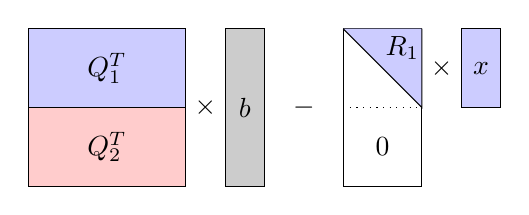
\begin{tikzpicture}

  \begin{scope}
  \filldraw[fill=blue!20] (0,1) rectangle (2,2);
  \filldraw[fill=red!20] (0,0) rectangle (2,1);
  \node at (1,1.5) {$Q_1^T$};
  \node at (1,0.5) {$Q_2^T$};
  \node at (2.25,1) {$\times$};
  \filldraw[fill=black!20] (2.5,0) rectangle (3.0,2);
  \node at (2.75,1) {$b$};
  \end{scope}

  \begin{scope}[shift={(4,0)}]
  \draw (0,0) rectangle (1,2);
  \draw[dotted] (0,1) -- (1,1);
  \filldraw[fill=blue!20] (0,2) -- (1,1) -- (1,2);
  \node at (0.75,1.75) {$R_1$};
  \node at (0.5,0.5)  {$0$};
  \node at (1.25,1.5) {$\times$};
  \draw[fill=blue!20] (1.5,1) rectangle (2.0,2);
  \node at (1.75,1.5) {$x$};
  \end{scope}

  \node at (3.5,1) {$-$};

\end{tikzpicture}
\end{document}
